\documentclass{article}
\usepackage{amsmath}
\usepackage{graphicx}
\usepackage{siunitx}
\usepackage{float}
\usepackage{gensymb}
\usepackage[dvipsnames]{xcolor}
\usepackage{sectsty}
\usepackage{indentfirst}
\usepackage{enumitem}

%\setlength{\parskip}{1em}

\definecolor{color:background}{RGB}{40,40,40}
\definecolor{color:text}{RGB}{230,230,230}

\pagecolor{color:background}
\color{color:text}
\allsectionsfont{\normalfont\sffamily\bfseries}

\title{STAT251 Elementary Statistics}
\author{Kelvin Hsu}


\begin{document}
    \sffamily
       \maketitle
       \newpage

    \section*{Normal Probability Approximations}
    \subsection*{Population and Sample}
    \begin{itemize}
        \item Population: The entire collection of individuals we want to study.
        \item Sample: A subset of individuals selected from the population.
    \end{itemize}

    Statistical techniques are used to make conclusions about the population 
    based on the sample.

    \subsection*{Statistic and Parameter}
    \begin{itemize}
        \item Statistic: A numerical summary of the sample. Ex. Sample mean, sample standard deviation.
        \item Sample: A numerical summary of the population. Ex. Population mean, population standard deviation.
    \end{itemize}

    Note that,
    \begin{itemize}
        \item Values of the parameter cannot be determined in practice.
        \item Due to sampling variability a statistic takes on different values for different samples.
        \item Parameters are estimated using sample date. Statistics is used to estimate parameters.
    \end{itemize}

    \subsection*{Sampling Distributions}
    The sampling distribution of a statistic is the probability distribution that specifies probabilities for the possible
    values the statistic can take.\par
    Sampling distributions describe the variability that occurs from study to study using statistics to estimate population parameters.\par
    Sampling distributions help to predict how close a statistic falls to the 
    parameter it estimates.

    If $X=[X_{1}, X_{2}, ... X_{n}]$ is a sample from a normal population with mean $\mu$ and 
    standard deviation $\sigma$, then

    \begin{equation*}
        \bar{X} = \frac{X_{1}+...X_{n}}{n} \sim N(\mu, \frac{\sigma^{2}}{n})
    \end{equation*}

    However, samples do not always follow a normal distribution. Suppose a random sample of 
    n observations is taken from a population with mean $\mu$ and standard deviation $\sigma$,
    then the mean of the mean of the samples is $\mu$ and the standard deviation of the mean of 
    the samples is $\frac{\sigma}{\sqrt{n}}$. The standard deviation of the samples mean is called the standard error.
    
    \section*{Central Limit Theorem}
    The CLT states that when an infinite number of successive random samples are taken from a population, the "sampling 
    distribution of the means of those samples will become approximately normally distributed with mean $\mu$ and 
    standard deviation $\frac{\sigma}{\sqrt{n}}$.

    Suppose we draw a random sample of size n, $X_{1}, X_{2}...X_{n}$ from a population random variable that is distributed
    with mean $\mu$ and standard deviation $\sigma$. Do this repeatedly and then calculate the mean of each sample. As the sample size
    increases, the distribution of the mean of the drawn samples will approach a normal distribution with mean $\mu$ and standard deviation $\frac{\sigma}{\sqrt{n}}$.


    \begin{equation*}
        \bar{X} = \frac{X_{1}+...X_{n}}{n} \sim N(\mu, \frac{\sigma^{2}}{n})
    \end{equation*}

    The central limit theorem describes how the population mean and standard deviation 
    are related to the mean and the standard deviation of the mean of the samples.

    Then,
    \begin{equation*}
        \frac{\bar{X}-\mu}{\frac{\sigma}{\sqrt{n}}} \sim N(0, 1)
    \end{equation*}

    \subsection*{Example}
    Closing prices of stocks have a right-skewed distribution with mean of $\$25$ and standard deviation of $\$20$.
    What is the probability that mean of a random sample of 40 stocks will be less than $\$20$?

    Consider the sampling distribution of sample mean. By CLT, 
    \begin{equation*}
        \bar{X} \sim N(25, \frac{20^{2}}{40})
    \end{equation*}

    \begin{align*}
        P(\bar{X} < 20) &= P(\frac{\bar{X} - \mu}{ \frac{\sigma}{\sqrt{n}}} < \frac{20-25}{\frac{20}{\sqrt{40}}})\\
        &= P(Z<-1.58)\\
        &= P(Z>1.58)\\
        &= 1-P(Z>1.58)\\
        &= 1-P(Z<1.58)\\
        &= \boxed{0.0571}
    \end{align*}

    \subsection*{Example}
    The time taken by a randomly selected applicant for a mortgage to fill out a certain form has a normal distribution
    with mean of 10 minute and standard deviation of 2 minute. If five individuals fill out a form on one day, what is the
    probability that the sample average amount of time taken on that day is at most 11 min?

    \begin{align*}
        &\mu = 10\\
        &\sigma = 2\\
        &n = 5\\
        &P(\bar{X} \leq 11) = ?
    \end{align*}

    \begin{align*}
        P(\bar{X} \leq 11) &= P(\frac{\bar{X} - \mu}{ \frac{\sigma}{\sqrt{n}}} \leq \frac{11-10}{\frac{2}{\sqrt{5}}})\\
        &=(Z\leq 1.12)\\
        &= 0.8686
    \end{align*}

    \section*{Normal Approximation to the Binomial Distribution}
    Let $X \sim Bin(n, p)$. When n is large so that both $np\geq 5$, we can use the normal distribution to 
    get an approximate answer.

    \begin{equation*}
        X \sim N(np, np(1-p))
    \end{equation*}

    * When we use normal approximation to the Binomial distribution, the \textbf{continuity correction} 
    should be used because we are approximating a discrete random variable with a continuous random variable.

    \subsection*{Example}
    Let $X \sim Bin(10, 0.5)$, obtain $P(x\leq 2)$,
    \begin{enumerate}
        \item exactly
        \item using the normal approximation
        \item using the normal approximation with a continuity correction
    \end{enumerate}

    \paragraph{1.}

    \begin{align*}
        &X \sim Bin(10, 0.5)\\
        &n = 10\\
        &p = 0.5
    \end{align*}

    \begin{align*}
        P(X \leq 2) &=  P(x = 0) + P(x = 1) + P(x = 2)\\
        & = {10 \choose 0 }(0.5)^{0}(0.5)^{10} + {10 \choose 1} (0.5)^{1}(0.5)^{9} + {10 \choose 2} (0.5)^{2}(0.5)^{8}\\
        & = 0.0547
    \end{align*}

    \paragraph{2.}
    \begin{align*}
        &n = 10\\
        &p = 0.5\\
        &np = 5 \geq 5\\
        &n(1-p) \geq 5
    \end{align*}

    Therefore $X \sim N(5, 2.5)$,

    \begin{align*}
        P(x\leq 2) &= P(\frac{x - \mu}{\sigma} \leq \frac{2-5}{\sqrt{2.5}})\\
        &= P(Z\leq-1.9) = 0.0287
    \end{align*}

    This is not so good because the exact answer is 0.0547.

    \paragraph{3.}

    \begin{align*}
        P(x \leq 2) &= P(x \leq 2 + 0.5) = P(\frac{x - \mu}{\sigma} \leq \frac{2.5-5}{\sqrt{2.5}})\\
        &= P(Z\leq-1.58)\\
        &= 0.0571
    \end{align*}
    
    0.5 is the continuity correction. The end result is closer to the exact answer.

    \section*{Continuity Correction}
    If x is a discrete random variable and y is a continuous random variable.
    \begin{align*}
        &P(x>4) = P(x\geq 5) = P(y \geq 4.5)\\
        &P(x \leq 4) = P(y \leq 4.5)\\
        &P(x<4) = P(x \leq 3) = P(y \leq3.5)\\
        &P(x \leq 4) = P(y \leq 4.5)\\
        &P(x = 4) = P(4-0.5 \leq y \leq 4+0.5)
    \end{align*}

    \section*{Normal Approximation To The Poisson Distribution}
    If $X \sim Poisson(\alpha)$ where $\alpha$ is the expected number of counts.
    When $\alpha$ is large ($\geq 20$), then normal distribution can be used to approximate the
    Poisson distribution.
    
    \begin{equation*}
        X \sim N(\alpha, \alpha)
    \end{equation*}
    
    \subsection*{Example}
    A radioactive element disintegrates such that it follows a Poisson distribution. The
    mean number of particles emitted is recoded in 1 second interval is 55. Find the probability of

    \begin{enumerate}[label={(\alph*)}]
        \item more than 60 particles are emitted in 1 second
        \item  between 50 and 65 particles inclusive are emitted in 1 second
    \end{enumerate}

    Let $X = \#$ of particles emitted in 1 second.
    \begin{equation*}
        X \sim Poisson(55)
    \end{equation*}

    Since $\lambda $ is large($\geq 20$), $X \sim N(55, 55)$.

    \paragraph{(a)}
    \begin{align*}
    P(X > 60) &= P(X \geq 61)\\
    &=P(X \geq 60.5)\\
    & = P(\frac{x-\mu}{\sigma} \geq \frac{60.5 - 55}{\sqrt{55}})\\
    & = P(Z \geq 0.74)\\
    & = 1 - P(Z < 0.74)\\
    & =1-0.7704\\
    & = 0.2296
    \end{align*}

    \paragraph*{(b)}
    \begin{align*}
        P(50 \leq x \leq 65) &= P(49.5 \leq x \leq 65.5)\\
        & = P(\frac{49.5-55}{\sqrt{55}} \leq \frac{x-\mu}{\sigma} \leq \frac{65.5-55}{\sqrt{55}})\\
        & = P(-0.74 \leq Z \leq 1.41)\\
        & = 0.6911
    \end{align*}

    \section*{Sum of Random Samples With CLT}
    Consider a random sample $X_{1}, X_{2}... X_{n}$ from a distribution with mean $\mu$ and variance
    $\sigma^{2}$. When n is large, by CLT

    \begin{equation*}    
          \bar{X} = \frac{X_{1}+...X_{n}}{n} \sim N(\mu, \frac{\sigma^{2}}{n})
    \end{equation*}

    If a question is about sum instead of an average, CLT can still be used.
    Let $T = X_{1} + X_{2} + .... X_{n}$,
    \begin{align*}
        E[T] = n\mu\\
        Var[T] = n\sigma^{2}\\
        T \sim N(n\mu, n\sigma^{2})
    \end{align*}

    \section*{Statistical Modeling and Inference}
    \subsection*{Statistical Inference}
    Method of making decisions or predictions about a population 
    based on information obtained from a sample.\par

    The objective of estimation is to determine the approximate value
    of a population parameter on the bases of a sample statistic.\par

    Sample mean ($\bar{X}$) is used to estimate the population mean($\mu$).\par

    \subsection*{Two Types of Estimators}
        \begin{itemize}  
            \item Point Estimator - draws inferences about a population 
                                    by estimating the value of an unknown parameter using a single value
                                    or point.
            \item Interval Estimator - draws inferences about a population
                                    by estimating the value of an unknown parameter using an interval.
                                    The population parameter of interest is between some lower and upper bounds.
        \end{itemize}

        \subsubsection*{Point Estimate vs Interval Estimate}
        A point estimate does not tell us how close the estimate is likely to be to the parameter.
        An interval estimate is usually more useful. 

    \section*{Point Estimators}
    A good estimator has a sampling distribution that
    is centered at the parameter(unbiasedness).\par

    An unbiased estimator of a population parameter is an estimator
    whose expected value is equal to that parameter.\par

    \begin{equation*}
        E[\hat{\theta}] = \theta
    \end{equation*}
    where $\theta$ is the parameter and $\hat{\theta}$ is a point estimator.\par

    A good estimator has a small standard error compared to the other estimators.\par

    \subsection*{Example}
    Suppose we want to estimate the mean summer income of a class of statistics students.
    For a sample of 30 students sample mean($\bar{X}$) is calculated to be $\$500$ per week.\par

    Point estimate for population mean($\mu$) income per week is $\hat{\mu} = \bar{X} = \$500$(point estimate).
    An alternative statement is: "The mean income is between $\$400 \sim \$600$ per week(interval estimate).

    \subsection*{Example}
    Suppose that $X_{1} , X_{2}... X_{n}$ is a random sample from a population with mean $\mu$
    and variance $\sigma^{2}$.\par
   
    \begin{itemize}
        \item $\bar{X}$ is an unbiased estimator of $\mu$
            \begin{equation*}
                E[\bar{X}] = E[\frac{\sum{X_{i}}}{n}] = \mu
            \end{equation*}
        \item $S^{2}$ is an unbiased estimator of $\sigma^{2}$
        \begin{equation*}
            E[S^{2}]  = \sigma^{2}
        \end{equation*}
    \end{itemize}

    \section*{Confidence Interval for $\mu$}
    Consider the absolute estimation error $|\bar{Y} - \mu|$ (sample mean - population mean). 
    We wish to find a value d such that there is a large probability (0.95 or 0.99) that the absolute estimation 
    error is below d.

    \begin{equation*}
        \text{Confidence Level} = P(|\bar{Y} - \mu| < d) = 1 - \alpha
    \end{equation*}
    where $\alpha$ is typically 0.05(95$\%$ confidence) or 0.01($99\%$ confidence). Assume 0.005 if not defined. \par

    The resulting d can be added or subtracted from the observed average $\bar{y}$ to obtain 
    the upper and lower limits of an interval called ($1-\alpha$) $100\%$ confidence interval.
    \begin{equation*}
        (\bar{y} - d, \bar{y} + d)
    \end{equation*}

    \subsection*{Example}
    \begin{align*}
        &\bar{X} \sim N(\mu, \frac{\sigma^{2}}{n})\\
        &Z = \frac{\bar{X} - \mu}{\frac{\sigma}{\sqrt{n}}}\\
        &P(-1.96 \leq \frac{\bar{X} - \mu}{\frac{\sigma}{\sqrt{n}}} \leq 1.96) = 0.95\\
        &P(\bar{X} - 1.96\frac{\sigma}{\sqrt{n}} \leq \mu \leq \bar{X} + 1.96\frac{\sigma}{\sqrt{n}}) = 0.95
    \end{align*}

    Therefore, 95$\%$ confidence interval for $\mu$ is 
    \begin{equation*}
        [\bar{X} - Z_{0.025}\frac{\sigma}{\sqrt{n}}, \bar{X} + Z_{0.025}\frac{\sigma}{\sqrt{n}}]
    \end{equation*}
    
    \subsection*{Example}
    The average zinc concentration recovered from a sample of measurements taken in 
    36 different locations in a river is found to be 2.6g per ml. Find the $95\%$ and $99\%$ confidence interval for 
    the mean zinc concentration in the river. Assume that the population standard deviation is 0.3g/ml.

    \begin{align*}
        \bar{X} = 2.6\\
        n = 36\\
        \sigma = 0.3
    \end{align*}

    \paragraph*{95$\%$ CI for $\mu$}
        \begin{align*}
            \bar{X} \pm Z_{\alpha/2} \frac{\sigma}{\sqrt{n}}\\
            [2.507, 2.693]
        \end{align*}

    \paragraph*{$99\%$ CI for $\mu$}
        \begin{equation*}
             [2.471, 2.729]
        \end{equation*}

    \section*{CI when $\sigma$ is unknown}
        $\sigma$ is estimated by the sample standard deviation S.
        This estimation introduces extra error. To account for this error,
        z-score is replaced by a slightly larger score called the t-score.

    \section*{Interpreting a CI for $\mu$}
    If we repeatedly obtain samples of size n and construct the corresponding $95\%$ 
    confidence interval for $\mu$, on average, $95\%$ of these intervals will include the value of $\mu$.

    \subsection*{Example}
    A reporter is writing an article on the cost of 
    off-campus housing. A sample of 16 studio apartments within 3 km of campus 
    resulted in a sample mean $\$1000/month$ and sample standard deviation of $\$150$.
    Assuming population to be normal, calculate $95\%$ CI for the population mean rent per month.

    \begin{align*}
        n = 16\\
        \bar{X} = 1000\\
        S = 150
    \end{align*}

    \begin{align*}
        \bar{X} \pm t_{0.025, n-1}\frac{s}{\sqrt{n}}\\
        1000 \pm 2.131 \frac{150}{\sqrt{16}}\\
        [920, 1080]
    \end{align*}

    \section*{Testing Hypothesis About $\mu$}
    Hypothesis testing can be used to determine whether 
    a statement about the value of a population parameter should or 
    should not be rejected.

    \section*{Null and Alternative Hypothesis}
    The null hypothesis, denoted by $H_{o}$, is a tentative assumption 
    about a population parameter.\par

    The alternative hypothesis, denoted by $H_{a}$ is the opposite of what is 
    stated in the null hypothesis. 
    The alternative hypothesis is what the test is attempting to establish. \par
    
    The equality part of the hypothesis always appears in the null hypothesis.\par

    Hypothesis test about the value of a population mean 
    $\mu$ must take one of the 3 forms.

    \begin{itemize}
        \item $H_{o}: \mu \geq \mu_{o} \text{ vs } H_{a}: \mu < \mu_{o}$
        \item $H_{o}: \mu \leq \mu_{o} \text{ vs } H_{a}: \mu > \mu_{o}$
        \item $H_{o}: \mu = \mu_{o} \text{ vs } H_{a}: \mu \neq \mu_{o}$
    \end{itemize}
    where $\mu_{o}$ is the hypothesized value of the population mean.\par

    The hypothesis should be formulated before viewing or analyzing the data.

    \section*{Test Procedures}
    A test procedures is specified by the following.

    \begin{itemize}
        \item Test Statistic: a function of the sample data on which the decision
        (Rejected $H_{o}$ or do not reject $H_{o}$) is to be based.
        \item Rejection Region: the set of all test statistic values for which $H_{o}$ will be rejected.
    \end{itemize}

    A test statistic is constructed assuming the null hypothesis is correct.

    \paragraph*{Case 1: $\sigma$ is known}
    test statistic is,
    \begin{equation*}
        Z = \frac{\bar{X} - \mu_{o}}{\frac{\sigma}{\sqrt{n}}} \sim N(0, 1)
    \end{equation*}

    \paragraph*{Case 2: $\sigma$ is unknown}
    test statistic is,
    \begin{equation*}
        t = \frac{\bar{X} - \mu_{o}}{\frac{s}{\sqrt{n}}} \sim t_{n-1}
    \end{equation*}
    When n is large,
    \begin{equation*}
        t = \frac{\bar{X} - \mu_{o}}{\frac{s}{\sqrt{n}}} \sim t_{n-1} \sim N(0,1)
    \end{equation*}

    The null hypothesis will be rejected if and 
    only if the observed or computed test statistic value falls in the rejection region.\par

    We also use the test statistic to assess the evidence against the 
    null hypothesis by giving a probability, p-value.

    \section*{P-Value}
    The P-Value summarizes the evidence. It describes how unusual the 
    data would be if $H_{o}$ were true.\par
    
    P-Value is defined as the probability of observing a result as extreme 
    or more extreme than what we observed given that $H_{o}$ is true.

    \section*{Significance Level ($\alpha$)}
    The Significance level is a predetermined number such that we reject $H_{o}$ if the P-Value 
    is less than or equal to that number.\par

    In practice, the most common significance level is $\alpha = 0.05$.\par

    When we reject $H_{o}$, we say the results are statistically significant.

    \begin{itemize}
        \item if $p-value \leq \alpha$ $=>$ Reject $H_{o}$
        \item if $p-value > \alpha$ $=>$ Do not reject $H_{o}$
    \end{itemize}

    \section*{Steps of Hypothesis Testing}
        \begin{enumerate}
            \item Develop the null and alternative hypothesis
            \item Specify the level of significance $\alpha$
            \item Collect the sample data and compute the test statistic
        \end{enumerate}

        Then, 2 approaches can be used.
        \paragraph*{p-value approach}
        \begin{enumerate}
            \item Use the value of the test statistic to compute the p-value
            \item Reject $H_{o}$ if $p-value \leq \alpha$
            \item Conclusion
        \end{enumerate}

        \paragraph*{Critical Value Approach}
        \begin{enumerate}
            \item Use the level of significance to determine the 
                    critical value and the rejection rule
            \item Use the value of the test statistic and rejection rule to determine whether to reject $H_{o}$
            \item Conclusion
        \end{enumerate}

        \section*{Decisions and Types of Errors in Hypothesis Testing}
        \begin{itemize}
            \item $H_{o}$ is true / Reject $H_{o}$ $=>$ type I error
            \item $H_{o}$ is false / Do not reject $H_{o}$ $=>$ type II error
        \end{itemize}

        \paragraph*{What is a good test?\newline}
        A test that rarely makes type I and type II errors.

        \begin{align*}
            \text{P(Type I error)} = \alpha \\
            \text{P(Type II error) }= \beta
        \end{align*}

        We can control the probability of type I error by our choice of the significance level $\alpha$.\par

        It is difficult to control the probability of making type II error.\par

        Statisticians avoid the risk of making a type II error by using "do not reject $H_{o}$" 
        and not "accept $H_{o}$"\par

        $1-\beta$  is referred to as the power of a test.The greater the power, 
        the less likely type II error occurs.\par

        $\alpha$ and $\beta$ are test properties, and they are independent of data.

        \section*{Power of a Test}
        Power is the probability of correctly rejecting the null hypothesis 
        $H_{o}$, when $H_{o}$ is false. 

        \section*{Tail Test}
        Use two tail test when $\mu = \mu_{o}$; use one tail test when $\mu \geq \mu_{o}$.
        \begin{figure}[H]
            \centering
            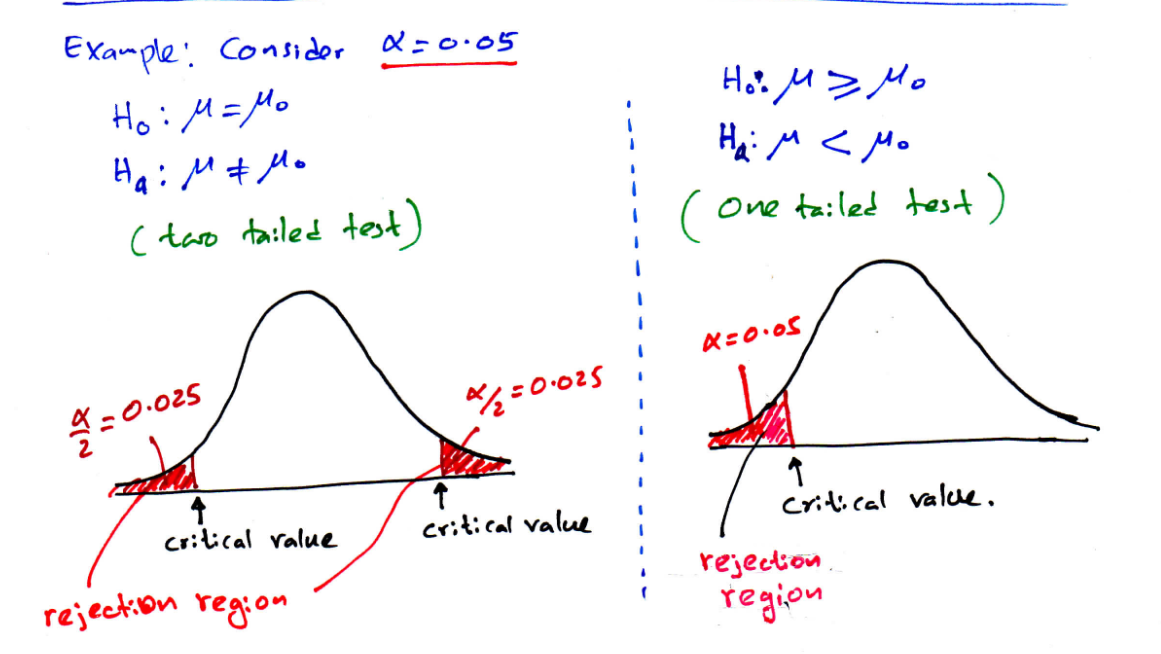
\includegraphics[width=10cm]{figures/tail_test.PNG}
            \caption{Tail Tests}
            \label{fig:tail_test}
        \end{figure}


        \subsection*{Example}
        A department store manager determines that a new billing system will be cost-effective 
        only if the mean monthly account is more then $\$170$.\par

        A random sample of 400 monthly accounts is drawn, from which the sample mean 
        is $\$178$. The accounts are approximately normally distributed with $\sigma = \$65$.

        \begin{enumerate}[label={(\alph*)}]
            \item Can we conclude that the new system will be cost effective? (use $\alpha = 0.05$)?
            \item Describe what type I and type II errors in the content of this problem situation
            \item Considering the test procedure, find the rejection region of $\bar{X}$
            \item When $\mu = 180$, find the probability of type II error.
            \item Evaluate the power of the test when $\mu = 180$
        \end{enumerate}

        \subsubsection*{(a)}
        \begin{align*}
            &n = 400\\
            &\bar{X} = 170\\
            &\sigma = 65
        \end{align*}

        \begin{align*}
            &H_{o} = \mu \leq 170  \rightarrow \text{ use right tail test}\\
            &\mu_{o} = 170\\
            &H_{a} = \mu > 170\\
        \end{align*}

        \begin{align*}
            Z_{obs} &= \frac{\bar{X}-\mu_{o}}{\frac{\sigma}{\sqrt{n}}} \sim N(0,1)\\
            &= \frac{178-170}{\frac{65}{\sqrt{400}}} = 2.46
        \end{align*}
        \paragraph*{Method1:Critical Value Approach}
        Since $Z_{obs}= 2.46 > Z_{0.05} = 1.645$, we reject $H_{o}$. The conclusion is that 
        the new system is cost-effective.\par
        
        \paragraph*{Method2:P-value Approach}
        P-Value = P(observing data as extreme or more extreme than what we observed, given $H_{o}$ is true)
        \begin{align*}
            P(\bar{X} \geq 178 \text{ when } \mu =  170)\\
            = P(Z \geq 2.46) = 0.0069
        \end{align*}
        Since $0.0069 < \alpha = 0.05$, $H_{o}$ is rejected, the conclusion is that the new system is cost 
        effective.

        \subsubsection*{(b)}

        Type I error: reject $H_{o}$ when $H_{o}$ is true.

        Conclude that the new billing system is cost-effective when it is not(i.e. true mean $>$ 170).\par

        Type II error: do not reject $H_{o}$ when $H_{o}$ is false.

        Conclude that the new billing system is not cost-effective when it is.

        \subsubsection*{(c)}
        Reject when $Z > 1.645$.
        \begin{align*}
            Z = \frac{\bar{X}- \mu_{o}}{\frac{\sigma}{\sqrt{n}}}\\
            \bar{X} > 175.35
        \end{align*}
        Therefore, rejection region is $\bar{X} > 175.35$.

        \subsubsection*{(d)}
        \begin{equation*}
            \mu = 180
        \end{equation*}
        When $\mu=180$, $\bar{X}$ has a normal distribution with mean 180 and sigma of $\frac{65}{\sqrt{400}}$.
        \begin{align*}
            \beta = \text{P(type II error)} &= \text{P(do not reject $H_{o}$ when $H_{o}$ is false)}\\
            &= P(\bar{X} < 175.35 \text{ when $\mu = 180$})\\
            &= P(\frac{\bar{X} - 180}{\frac{65}{\sqrt{400}}} < \frac{175.35 - 180}{\frac{65}{\sqrt{400}}})\\
            &= P(Z < -1.43)\\
            &= 0.0764
        \end{align*}

        \subsubsection*{(e)}
        \begin{align*}
            \text{Power} &= \text{P(Reject $H_{o}$ when $H_{o}$ is false)}\\
            &= 1-\beta\\
            &= 1-0.0764\\
            &= 0.9236
        \end{align*}
        This is a very powerful test since it makes the correct decision 92.36$\%$ of the time when $\mu = 180$.

        \section*{Two Sample Problems}
        Compare the means of two independent populations, assuming equal population standard deviations.\par

        *Suppose we draws a random sample from each of the two independent populations 
        with means $\mu_{1}$, $\mu_{2}$, and standard deviations of $\sigma_{1}$ and $\sigma_{2}$.\par

        Hypotheses take one of the following 3 forms.
        \begin{itemize}
            \item Left-Tailed
                \begin{align*}
                    H_{o}: \mu_{1} -  \mu_{2} \geq \Delta_o\\
                    H_{a}: \mu_{1} -  \mu_{2} < \Delta_o
                \end{align*}
            \item Right-Tailed
                \begin{align*}
                    H_{o}: \mu_{1} -  \mu_{2} \leq \Delta_o\\
                    H_{a}: \mu_{1} -  \mu_{2} > \Delta_o
                \end{align*}
            \item Two-Tailed
                \begin{align*}
                    H_{o}: \mu_{1} -  \mu_{2} = \Delta_o\\
                    H_{a}: \mu_{1} -  \mu_{2} \neq \Delta_o
                \end{align*}
        \end{itemize}

        \subsection*{Example}

        If the Hypotheses are
            \begin{align*}
                H_{o}: \mu_{1} \geq  \mu_{2} \rightarrow \mu_{1} - \mu_{2} \geq 0\\
                H_{a}: mu_{1} <  \mu_{2}  \rightarrow \mu_{1} - \mu_{2} < 0
            \end{align*}
        In this case, $\Delta = 0$.

        \subsection*{Assumptions}
        \begin{itemize}
            \item random samples from each of the population is drawn
            \item the sample individuals are independent of each other
            \item both populations are normal or we need reasonably large samples to validate using CLT
            \item both population distributions have equal variance ($\sigma_{1}^{2} = \sigma_{2}^{2}$)
        \end{itemize}
       
        \subsection*{Test Statistic}
        We select a simple random sample of size $n_{1}$, from population 1 and a simple random sample 
        of size $n_{2}$.\par
        Let $\bar{X_{1}}$ be the mean of sample 1 and $\bar{X_{2}}$ be the mean of sample 2.\par

        Test statistic t is.
        \begin{equation*}
            t = \frac{(\bar{X_{1}} - \bar{X_{2}})-\Delta_{o}}{S_{p} \sqrt{\frac{1}{n_{1}}+\frac{1}{n_{2}}}}
        \end{equation*}
        where $S_{p}$ is the pooled standard deviation.

        \subsection*{The Pooled Standard Deviation}
        This method requires the assumption that population variances are equal.
        \begin{equation*}
            \sigma_{1}^{2} =  \sigma_{2}^{2} =  \sigma^{2}
        \end{equation*}

        $S_{p}$, the pooled standard deviation estimates the common value $\sigma$.
        \begin{equation*}
            S_{p} = \sqrt{\frac{(n_{1}-1)S_{1}^{2}+(n_{2} - 1) S_{2}^{2}}{n_{1}+n_{2} -2}}
        \end{equation*}

        $(1-\alpha)100\%$ confidence interval for the difference between two population means (i.e. $\mu_{1} - \mu_{2}$).\par

        \begin{itemize}
            \item Point Estimator of $\mu_{1} - \mu_{2}$ is $\bar{X_{1}} - \bar{X_{2}}$
            \item CI $\rightarrow$ point estimate $\pm$ margin of error.
            \item $(1-\alpha)100\%$ CI for $\mu_{1} - \mu_{2}$ is 
                  \begin{equation*}
                    (\bar{X_{1}}- \bar{X_{2}}) \pm t_{\frac{\alpha}{2}, n_{1} + n_{2} - 2} \cdot S_{p} \cdot \sqrt{\frac{1}{n_{1}}+\frac{1}{n_{2}}}
                  \end{equation*}
        \end{itemize}

        \subsection*{Example}
        Average densities of two types of brick are compared. (Type A and Type B).
        \subsubsection*{a)}
        Using the following sample data, test the claim that the 
        true mean densities are equal.
        \subsubsection*{b)}
        Use a 0.05 significance level and assume normality of the two density distribution and equal population variances.
        \subsubsection*{c)}
        Calculate $95\%$ CI for $\mu_{A} - \mu_{B}$.

        \begin{center}
            \begin{tabular}{c c}
            Type A & Type B   \\
            $n_{A} = 8$ & $n_{B} = 10$ \\
            $\bar{X_{A}} = 22.7$ & $\bar{X_{B}} = 21.5$ \\
            $S_{A} = 0.8$ & $S_{B} = 0.6$
            \end{tabular}
        \end{center}

        Let $\mu_{A}$ be the true average density for type A and $\mu_{B}$
        be the true density for Type B.

        \subsubsection*{Hypotheses}
            \begin{align*}
                H_{o}: \mu_{A} = \mu_{B} \rightarrow \mu_{A} - \mu_{B} = 0\\
                H_{a}: \mu_{A} \neq \mu_{B}  \rightarrow \mu{A} = \mu_{B} \neq 0
            \end{align*}
            Use two tail test and $\alpha = 0.05$.

        \subsubsection*{Pooled Standard Deviation}
            \begin{align*}
                S_{p}^{2} &= \frac{ (n_{A} - 1)S_{A}^{2} + (n_{B} - 1) S_{B}^{2} }{n_{A} + n_{B} - 2}\\
                &=  \frac{ (8 - 1)(0.8)^{2} + (10 - 1) (0.6)^{2} }{8 + 10 - 2}\\
                &= 0.4825\\
                &S_{p} = 0.695
            \end{align*}
        \subsubsection*{Test Statistic}
             \begin{align*}
                t_{obs} &= \frac{(\bar{X_{A}} - \bar{X_{B}})-0}{S_{p} \sqrt{\frac{1}{n_{A}}+\frac{1}{n_{B}}}} \sim t_{n_{1}+n_{2}-2}\\
                &= \frac{22.7-21.5}{0.695 \sqrt{\frac{1}{8} +\frac{1}{10}}}\\
                &= 3.64
             \end{align*}
       \subsubsection*{Critical Value Approach} 
       \begin{align*}
        &\alpha = 0.05\\
        &\alpha/2 = 0.025\\
        &t_{0.025, 16} = 2.12\\
       \end{align*}

       Calculated test statistic value is in the rejection region.
       \begin{equation*}
        |t_{obs}| = 3.64 > t_{0.025, 16} = 2.12 \rightarrow \text{Reject } H_{o} \text{ at } \alpha = 0.05
       \end{equation*}

       \subsubsection*{Conclusion}
       At the significant level 0.05, we conclude that 
       the true mean densities of two types of brick are not equal.

       \subsubsection*{c)}
            \begin{align*}
                &(\bar{X_{A}}- \bar{X_{B}}) \pm t_{\frac{\alpha}{2}, n_{A} + n_{B} - 2} \cdot S_{p} \cdot \sqrt{\frac{1}{n_{A}}+\frac{1}{n_{B}}}\\
                &(22.7 - 21.5) \pm 2.12 (0.695) \sqrt{\frac{1}{8}+\frac{1}{10}}\\
                &1.2 \pm 0.33\\
                &[0.87, 1.53]
            \end{align*}

        \subsubsection*{Hypotheses}
            \begin{align*}
                H_{o}: \mu_{A} - \mu_{B} = 0\\
                H_{a}: \mu_{A} - \mu_{B} \neq 0
            \end{align*}

            The calculated confidence interval does not contain the hypothesized value.
            Therefore we can reject the null hypothesis, $H_{o}$.

            \section*{Comparison of Several Means}
            \subsection*{Analysis of Variance ANOVA}
            ANOVA is a statistical method that tests the equality of three or more population 
            means by analyzing sample variances or variation in the data.\par
            he simplest ANOVA problem is referred to variously as a single-factor, single-classification, 
            or one-way ANOVA.

            \subsection*{Example}
            \begin{enumerate}
                \item An experiment to study the effect of five different brands of gasoline 
                        on automobile engine operating efficiency (mpg)
                \item An experiment to study the effect of the presence of three 
                        different sugar solutions on bacterial growth.
            \end{enumerate}

            \subsection*{One-Way ANOVA}
            One-way ANOVA focuses on a comparison of 3 or more population or 
            treatment means.\par

            Let k be the number of populations or treatments being compared.
            \begin{align*}
                &\mu_{1} \text{ is the mean of population 1 or the true average response when 
                treatment 1 is applied.}\\
                &\text{.}\\
                &\text{.}\\
                &\text{.}\\
                &\mu_{k} \text{ is the mean of population k or the true average 
                response when treatment k is applied.}
            \end{align*}

            \subsection*{Hypotheses}
            \begin{align*}
                H_{o}: \mu_{1} = \mu_{2} = ...= \mu_{k}\\
                H_{a}: \text{at least two of the $\nu_{i}$ are different}
            \end{align*}
            Reject $H_{o}$ here means that at least two population means have 
            different values.

            \subsection*{Assumptions for ANOVA}
            For each population, the response variable is normally distributed.\par
            The variance of the response variable, denoted $\sigma^{2}$, is the same for all the 
            populations.\par
            The observations must be independent.
            
            \subsection*{Notation}
            k random samples observed.
            $y_{ij}$ is the $j_{th}$ observed value from the $i^{th}$ population.

            \begin{figure}[H]
                \centering
                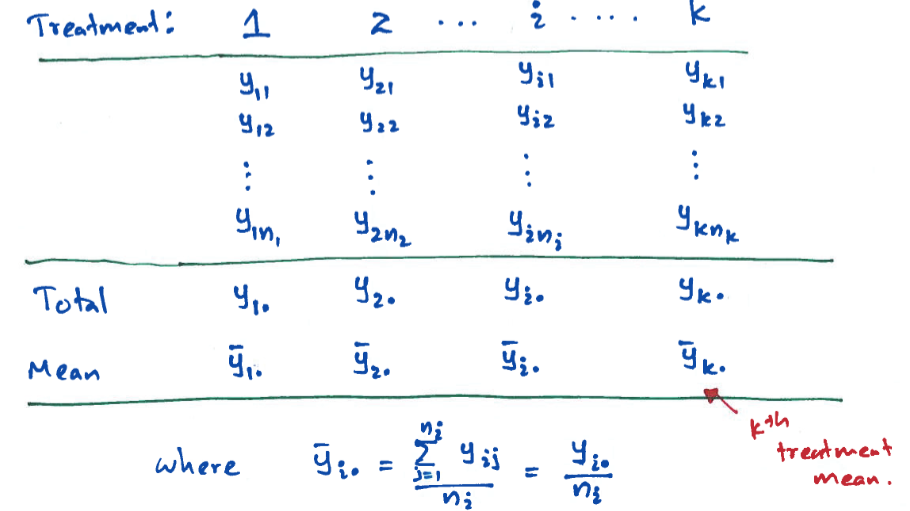
\includegraphics[width=10cm]{figures/anova_table.PNG}
                \label{fig:anova_table}
            \end{figure}

            where,
            \begin{equation*}
                \bar{y_{i}} = \frac{\sum_{j=1}^{ni} y_{ij}}{n_{i}} = \frac{y_{i0}}{n_{i}}
            \end{equation*}

            \begin{align*}
                \text{Total Sample Size } = n = n_{1} + ...n_{k}\\
                \text{Grand Total } = y_{oo} = \sum_{k}^{i = 1} \sum_{n_{i}}^{j=1}y_{ij}\\
                \text{Grand Mean } = \bar{y_{oo}} = \frac{y_{oo}}{n} = \frac{\sum_{k}^{i = 1} \sum_{n_{i}}^{j=1}y_{ij}}{n} 
            \end{align*}

            Let $Y_{ij}$ be the random variable that denotes the $j^{th}$ measurement 
            taken from the $i^{th}$ treatment.

            Then $y_{ij}$ is the observed value of $Y_{ij}$.

            \begin{align*}
                E[\bar{y_{i}}] = \mu_{i}\\
                Var(\bar{y_{i}}) = \frac{\sigma}{n_{i}}
            \end{align*}

            For k random samples, we can find calculate the sample variances.
            \begin{equation*}
                S_{1}^{2}, S_{2}^{2}...S_{k}^{2}
            \end{equation*}

            $S_{1}^{2}, S_{2}^{2}...S_{k}^{2}$ are k different 
            unbiased estimates for the common variance $\sigma^{2}$.
            \begin{equation*}
                E[S_{i}^{2}] = \sigma^{2}
            \end{equation*}
          
            These k estimates can be combined to obtain an 
            unbiased estimate for $\sigma^{2}$.
            \begin{equation*}
                s^{2} = \frac{\sum_{i=1}^{k} (n_{i}-1)S_{i}^{2}}{n-k} = MSE
            \end{equation*}
            where
            \begin{equation*}
                S_{i}^{2} = \frac{\sum_{i=1}^{n_{i}} (y_{ij} - \bar{y_{ij}})^{2}}{n_{i} - 1}
            \end{equation*}

            \subsection*{$H_{o}$ is true}
            Sample means are close together because there is only one sampling distribution.

            \subsection*{$H_{o}$ is false}
            Sample means comes from different sampling distributions and are not close together.

            \subsection{Total Variation In The Data (SSE - total sum of squares)}
            Comes from 2 sources.
            \begin{itemize}
                \item Variation between groups/treatments. (SSTr- Treatment sum of squares)
                \item Variation within groups/treatments.(SSE - Error sum of squares)
            \end{itemize}

            \begin{equation*}
                SST = SSTr + SSE
            \end{equation*}

            \begin{align*}
                &SST = \sum_{i=1}^{k}\sum_{j=1}^{n_{i}} (y_{ij}- \bar{y_{oo}})^{2} =  \sum_{i=1}^{k}\sum_{j=1}^{n_{i}}  y_{ij}^{2} - \frac{1}{n}y_{oo}^{2}\\
                &SSTr = \sum_{i=1}^{k}\sum_{j=1}^{n_{i}} (\bar{y_{io} - \bar{y_{oo}}})^{2} =  \sum_{i=1}^{k} \frac{1}{n_{i}} y_{i}^{2} - \frac{1}{n} y_{oo}^{2}\\
                &SSE =  \sum_{i=1}^{k}\sum_{j=1}^{n_{i}} (y_{ij} - \bar{y_{io}})^{2} =  \sum_{i=1}^{k}\sum_{j=1}^{n_{i}} y_{ij}^{2} - \sum_{i=1}^{k} \frac{y_{io}^{2}}{n_{i}} = \sum_{i=1}^{k} (n_{i} - 1)S_{i}^{2}
            \end{align*}

            \subsection*{Degrees of Freedom}
            \begin{align*}
                df(SST) = n-1\\
                df(SSE) = n-k\\
                df(SSTr) = k-1
            \end{align*}

            \subsection*{Mean Squares}
            \begin{align*}
                \text{Mean Square Treatment} = MSTr = \frac{SSTr}{k-1}\\
                \text{Mean Square Error} = MSE = \frac{SSE}{n-k}
            \end{align*}
            *MSE is a measure of with-sample variation.

            \subsection*{ANOVA Test Procedure}
            \begin{align*}
                &H_{o}: \mu_{1} = \mu_{2} = \dots = \mu_{k}\\
                &H_{a}: \mu_{i} \neq \mu_{j} \text{ for } i\neq j
            \end{align*}

            \subsection*{Test Statistic}
            \begin{equation*}
                F_{obs} = \frac{MSTr}{MSE} \sim F_{\gamma_{1}, \gamma_{2}}
            \end{equation*}

            Under $H_{o}$, $F_{obs}$ follows the F-distribution with degrees of freedom,
            \begin{align*}
                \gamma_{1}(\text{numerator df}) = df(SSTr) = k-1\\
                \gamma_{2}(\text{Denominator df} = df(SSE) = n-k
            \end{align*}
            \subsection*{F-distribution}
            Reject $H_{o}$ if $F_{obs} \geq F_{\alpha}$.

            \subsection*{The ANOVA TABLE}
            \begin{figure}[H]
                \centering
                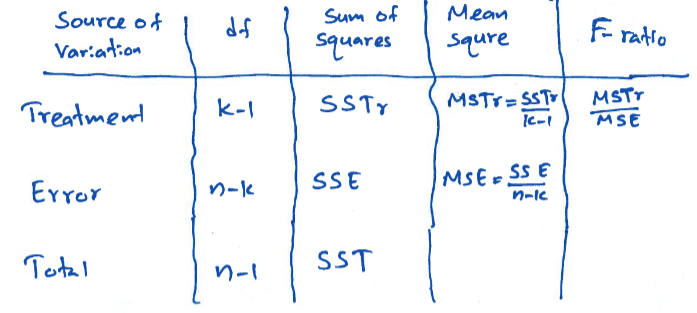
\includegraphics[width=10cm]{figures/anova_table2.PNG}
                \label{fig:anova_table2}
            \end{figure}
          
            \subsection*{The ANOVA Model}
            The assumptions of single-factor ANOVA can be described sufficiently 
            by means of the "model equation". \par
            Each measurement will be represented as the sum of 
            two terms, as unknown constant, $\mu_{i}$, and a random variable, $\epsilon_{ij}$.

            \begin{align*}
                &Y_{ij} = \mu_{i} + \epsilon_{ij}\\
                &i = 1, 2, \dots , k\\
                &j = 1, 2, \dots ,n_{i}
            \end{align*}
            where $\epsilon_{ij}$ represents a random deviation from the population or true treatment 
            mean $\mu_{i}$.

            \subsection*{The model assumptions are:}
            \begin{enumerate}
                \item Independence: The random variables $\epsilon_{ij}$ are independent (implying that $X_{ij}$ are also).
                \item Constant Treatment Means: $E(\epsilon_{ij}) = 0$ for all i and j
                \item Constant Variance: $Var(\epsilon_{ij}) = \sigma^{2}$ for all i and j
                \item Normality: The variables $\epsilon_{ij}$ are normal.
            \end{enumerate}
            


\end{document}

 